\tikzset{every picture/.style={line width=0.75pt}} %set default line width to 0.75pt        

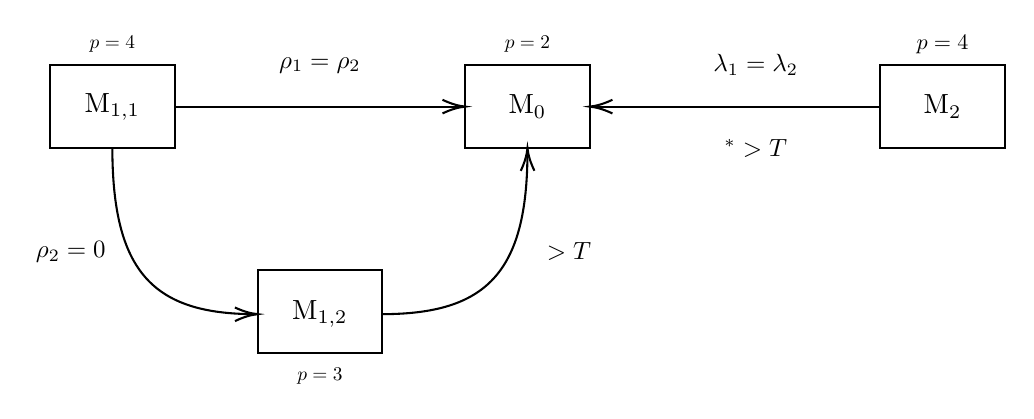
\begin{tikzpicture}[x=0.75pt,y=0.75pt,yscale=-1,xscale=1]
%uncomment if require: \path (0,269.6363525390625); %set diagram left start at 0, and has height of 269.6363525390625

\draw    (100, 80) rectangle (160, 120)   ;
\draw    (300, 80) rectangle (360, 120)   ;
\draw    (200, 178.67) rectangle (260, 218.67)   ;
\draw    (160,100) -- (298,100) ;
\draw [shift={(300,100)}, rotate = 180] [color={rgb, 255:red, 0; green, 0; blue, 0 }  ][line width=0.75]    (10.93,-3.29) .. controls (6.95,-1.4) and (3.31,-0.3) .. (0,0) .. controls (3.31,0.3) and (6.95,1.4) .. (10.93,3.29)   ;

\draw    (260,200) .. controls (309.86,199.95) and (329.96,180.35) .. (330,121.79) ;
\draw [shift={(330,120)}, rotate = 449.65] [color={rgb, 255:red, 0; green, 0; blue, 0 }  ][line width=0.75]    (10.93,-3.29) .. controls (6.95,-1.4) and (3.31,-0.3) .. (0,0) .. controls (3.31,0.3) and (6.95,1.4) .. (10.93,3.29)   ;

\draw    (130,120) .. controls (130.07,179.67) and (149.68,199.87) .. (198.51,200) ;
\draw [shift={(200,200)}, rotate = 539.6800000000001] [color={rgb, 255:red, 0; green, 0; blue, 0 }  ][line width=0.75]    (10.93,-3.29) .. controls (6.95,-1.4) and (3.31,-0.3) .. (0,0) .. controls (3.31,0.3) and (6.95,1.4) .. (10.93,3.29)   ;

\draw    (500, 80) rectangle (560, 120)   ;
\draw    (362,100) -- (500,100) ;

\draw [shift={(360,100)}, rotate = 0] [color={rgb, 255:red, 0; green, 0; blue, 0 }  ][line width=0.75]    (10.93,-3.29) .. controls (6.95,-1.4) and (3.31,-0.3) .. (0,0) .. controls (3.31,0.3) and (6.95,1.4) .. (10.93,3.29)   ;

\draw (130,100) node  [align=left] {M$_{1,1}$};
\draw (330,100) node  [align=left] {M$_{0}$};
\draw (230,200) node  [align=left] {M$_{1,2}$};
\draw (230,80) node [scale=0.9]  {$\rho _{1} =\rho _{2}$};
\draw (110,170) node [scale=0.9]  {$\rho _{2} =0$};
\draw (350,170) node [scale=0.9]  {$\uptau  >T$};
\draw (130,70) node [scale=0.7] [align=left] {$p=4$};
\draw (330,70) node [scale=0.7] [align=left] {$p=2$};
\draw (230,230) node [scale=0.7] [align=left] {$p=3$};
\draw (530,100) node  [align=left] {M$_{2}$};
\draw (440,80) node [scale=0.9]  {$\lambda_{1} =\lambda_{2}$};
\draw (440,120) node [scale=0.9]  {$\uptau^* >T$};
\draw (530,70) node [scale=0.8] [align=left] {$p=4$};


\end{tikzpicture}
